\documentclass{article}

\usepackage{amsmath, amsthm, amssymb, amsfonts}
\usepackage{thmtools}
\usepackage{graphicx}
\usepackage{setspace}
\usepackage{geometry}
\usepackage{float}
\usepackage[backend=biber,style=ieee,sorting=ynt]{biblatex}
\usepackage[hidelinks]{hyperref}
\usepackage[utf8]{inputenc}
\usepackage[spanish]{babel}
\usepackage{framed}
\usepackage[dvipsnames]{xcolor}
\usepackage{tcolorbox}
\usepackage{tikz}
\usetikzlibrary{positioning}
\usetikzlibrary{arrows.meta}
\usepackage{caption}
\usepackage{longtable}
\usepackage{pdflscape}
\usepackage{svg}
\usepackage{subcaption}
\usepackage{caption}
\usepackage{multirow}
\usepackage{array}
\usepackage{listings}
\usepackage{cancel}
\usepackage{fancyhdr}

\addbibresource{referencias.bib}


\colorlet{LightGray}{White!90!Periwinkle}
\colorlet{LightOrange}{Orange!15}
\colorlet{LightGreen}{Green!15}



\newcommand{\HRule}[1]{\rule{\linewidth}{#1}}

\declaretheoremstyle[name=Theorem,]{thmsty}
\declaretheorem[style=thmsty,numberwithin=section]{theorem}
\tcolorboxenvironment{theorem}{colback=LightGray}

\declaretheoremstyle[name=Proposition,]{prosty}
\declaretheorem[style=prosty,numberlike=theorem]{proposition}
\tcolorboxenvironment{proposition}{colback=LightOrange}

\declaretheoremstyle[name=Principle,]{prcpsty}
\declaretheorem[style=prcpsty,numberlike=theorem]{principle}
\tcolorboxenvironment{principle}{colback=LightGreen}

\newcolumntype{L}[1]{>{\raggedleft\let\newline\\\arraybackslash\hspace{0pt}}m{#1}}
\newcolumntype{C}[1]{>{\centering\let\newline\\\arraybackslash\hspace{0pt}}m{#1}}
\newcolumntype{R}[1]{>{\raggedright\let\newline\\\arraybackslash\hspace{0pt}}m{#1}}

\hypersetup{
    pdftitle={My Document Title},
    pdfauthor={Ludwig Alvarado},
    pdfsubject={Descripción del documento},
    pdfkeywords={palabras, interesantes},
    pdfcreator={GNU Emacs desde Arch GNU/Linux (btw) y LaTeX con hyperref},
    pdfproducer={pdflatex}
}


\setstretch{1.2}
\geometry{
    textheight=9in,
    textwidth=5.5in,
    top=1in,
    headheight=12pt,
    headsep=25pt,
    footskip=30pt
}

\lstdefinestyle{bashstyle}{
    language=bash,
    basicstyle=\ttfamily,
    backgroundcolor=\color{gray!10},
    keywordstyle=\color{blue},
    commentstyle=\color{green!40!black},
    stringstyle=\color{red},
    showstringspaces=false,
    numbers=left,
    numberstyle=\tiny\color{gray},
    breaklines=true,
    breakatwhitespace=true,
    frame=tb,
    rulecolor=\color{black!70},
    framerule=0.5pt,
    tabsize=4,
    captionpos=b
}

\lstdefinestyle{javastyle}{
    language=Java,
    basicstyle=\ttfamily,
    backgroundcolor=\color{gray!10},
    keywordstyle=\color{blue},
    commentstyle=\color{green!40!black},
    stringstyle=\color{red},
    showstringspaces=false,
    numbers=left,
    numberstyle=\tiny\color{gray},
    breaklines=true,
    breakatwhitespace=true,
    frame=tb,
    rulecolor=\color{black!70},
    framerule=0.5pt,
    tabsize=4,
    captionpos=b
}

\lstdefinestyle{pythonstyle}{
    language=Python,
    basicstyle=\ttfamily,
    backgroundcolor=\color{gray!10},
    keywordstyle=\color{blue},
    commentstyle=\color{green!40!black},
    stringstyle=\color{red},
    showstringspaces=false,
    numbers=left,
    numberstyle=\tiny\color{gray},
    breaklines=true,
    breakatwhitespace=true,
    frame=tb,
    rulecolor=\color{black!70},
    framerule=0.5pt,
    tabsize=4,
    captionpos=b
}

\lstdefinestyle{cppstyle}{
    language=C++,
    basicstyle=\ttfamily,
    backgroundcolor=\color{gray!10},
    keywordstyle=\color{blue},
    commentstyle=\color{green!40!black},
    stringstyle=\color{red},
    showstringspaces=false,
    numbers=left,
    numberstyle=\tiny\color{gray},
    breaklines=true,
    breakatwhitespace=true,
    frame=tb,
    rulecolor=\color{black!70},
    framerule=0.5pt,
    tabsize=4,
    captionpos=b
}



\pagestyle{fancy}
\fancyhf{}
\renewcommand{\headrulewidth}{0pt}
\fancyfoot[C]{\thepage}
\fancyfoot[C]{\footnotesize \thepage \quad \textbar{} \quad Este trabajo está bajo una licencia CC BY-SA 4.0.\\ Más info: \url{https://creativecommons.org/licenses/by/4.0/}}


% ------------------------------------------------------------------------------

\begin{document}

% ------------------------------------------------------------------------------
% Cover Page and ToC
% ------------------------------------------------------------------------------

\title{ \normalsize \textsc{}
	\\ [2.0cm]
	\HRule{1.5pt} \\
	\LARGE \textbf{\uppercase{Nombre Materia}
		\HRule{2.0pt} \\ [0.6cm] \LARGE{Universidad de Bogotá Jorge Tadeo Lozano} \vspace*{13\baselineskip}}
}
\date{}
\author{\textbf{\href{https://github.com/GNUTADEO/Rafiki}{GNUTADEO/Rafiki}} \\
	 }

\maketitle
\thispagestyle{empty}
\newpage

\tableofcontents
\listoffigures
\listoftables
\thispagestyle{empty}
\newpage
\setcounter{page}{1}

\section{Nombre del tema}

Aquí debes explicar el tema que quieres tratar que sea de la asignatura. Si quieres insertar fórmulas matemáticas lo puedes hacer con el bloque de \texttt{align}, por ejemplo:

\begin{align}
  E &= mc^2 \\
  y &= mx + b
\end{align}

Si no la quieres enumerar, puedes usar \texttt{align*}

\begin{align*}
  E &= mc^2 \\
  y &= mx + b
\end{align*}


Para insertar figuras recomendamos guardar todo en el directorio de \texttt{img/} y utilizar \texttt{figure} para insertar las imágenes como se muestra ne la figura~\ref{fig:cabito}.

\begin{figure}[H]
  \centering
  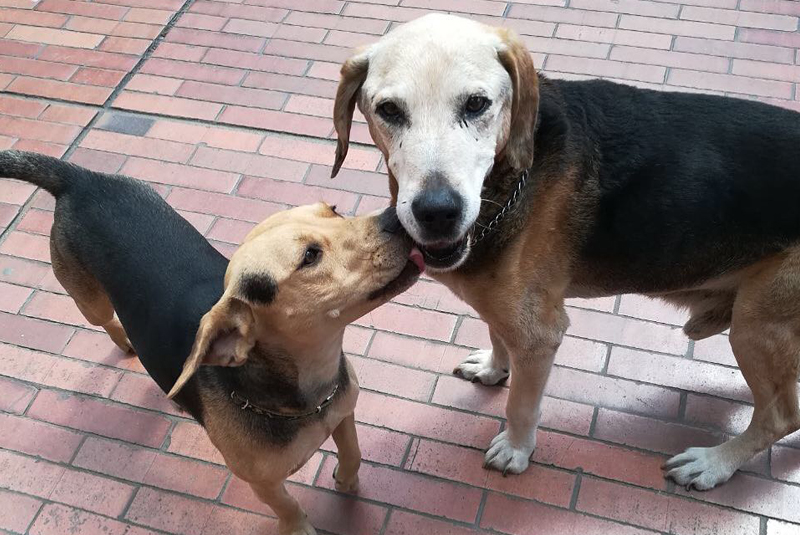
\includegraphics[width=0.8\textwidth]{img/Cabito.jpg}
  \caption{Cabito chévere!}
  \label{fig:cabito}
\end{figure}

Para tablas si es corta, recomendamos usar \texttt{table} como se muestra en el cuadro


\begin{table}[H]
  \centering
  \begin{tabular}{|c|c|c|}
    \hline
    Ejemplo & Ejemplo & Ejemplo \\ \hline
    1 & 2 & 3 \\ \hline
    4 & 5 & 6 \\ \hline
  \end{tabular}
  \caption{Tabla de ejemplo}
  \label{tab:tabla-ejemplo}
\end{table}


\addcontentsline{toc}{section}{Referencias}
\printbibliography

\newpage

\thispagestyle{empty}

\vspace*{0.3\textwidth}

\begin{figure}[H]
  \centering
  \includesvg[width=\textwidth]{img/LogoUtadeo.svg}
\end{figure}



\end{document}
